\documentclass[12pt, twoside]{article}

% Bibliography.
\usepackage{cite}

\newcommand{\reporttitle}{\textit{hp-Adaptive} Discontinuous Galërkin Algorithms}
\newcommand{\accentcolor}{solarized-red}
\newcommand{\urlcolor}{solarized-yellow}

\usepackage{amsmath}
\usepackage{mathrsfs}
\usepackage{amsthm}
\usepackage{amsfonts}
\usepackage{bm}
\usepackage{amssymb}
\usepackage{stmaryrd}

% Sets and spaces.
\newcommand{\R}{\mathbb{R}}
\newcommand{\RT}{\mathbb{R}^2}
\newcommand{\N}{\mathbb{N}}

\newcommand{\PK}[1]{\mathbb{P}_{#1}}

\newcommand{\LT}{\mathscr{L}^2}
\newcommand{\HO}{\mathscr{H}^1}

\newcommand{\Tau}{\mathcal{T}}
\newcommand{\F}{\mathcal{F}}

% Vectors and operators.
\newcommand{\Vector}[1]{\bm{#1}}
\newcommand{\Operator}[1]{\textcolor{solarized-cyan}{#1}}

% Matrices.
\newcommand{\MA}{\mathcal{A}}
\newcommand{\VB}{\mathcal{B}}

% Gradient and divergence.
\newcommand{\grad}{\Vector{\nabla}}
\newcommand{\diver}{\text{div }}

% Span.
\newcommand{\Span}[1]{\text{span} \left\{ #1 \right\}}

% Bilinear operators.
\newcommand{\boa}[2]{\Operator{a}(#1, #2)}

% Redefinition.
\newcommand{\Exists}{\exists ~}
\newcommand{\Forall}{\forall ~}

% Theorems.
\newtheorem{theorem}{Theorem}[section]
\newtheorem{lemma}{Lemma}[section]
\newtheorem{proposition}{Proposition}[section]

\newtheorem*{theorem*}{Theorem}

\usepackage{courier}
\usepackage{listings}

\lstdefinestyle{default}{
	basicstyle=\ttfamily\color{solarized-base01},
	breakatwhitespace=false,
	breaklines=true,
	keepspaces=true,
	showspaces=false,
	showstringspaces=false,
	showtabs=false,
	tabsize=2
}

\lstdefinestyle{cpp}{ % C++
	commentstyle=\color{solarized-green},
	keywordstyle=\color{solarized-blue},
	stringstyle=\color{solarized-orange},
	basicstyle=\ttfamily\color{solarized-base02},
	numberstyle=\ttfamily\color{solarized-base01},
	breakatwhitespace=false,
	breaklines=true,
	captionpos=b,
	keepspaces=true,
	showspaces=false,
	language=c++,
	showstringspaces=false,
	showtabs=false,
	numbers=left,
	tabsize=4
}

\lstset{style=default}

\usepackage{nameref}
\usepackage{multicol}
\usepackage{titlesec}

\usepackage{enumerate}

\usepackage{graphicx}
\graphicspath{{gallery/}}

\usepackage{xcolor-solarized}
\color{solarized-base02}

\usepackage[T1]{fontenc}
\usepackage[utf8]{inputenc}

\usepackage[a4paper]{geometry}
\geometry{
	inner=20mm,
	outer=20mm,
	top=30mm,
	bottom=30mm,
	heightrounded,
	marginparwidth=50pt,
	marginparsep=20pt,
	headsep=25pt,
	headheight=30pt
}

\usepackage{hyperref}
\hypersetup{
	linktocpage=true,
	colorlinks=true,
	linkcolor=\accentcolor,
	urlcolor=\urlcolor,
	citecolor=\accentcolor,
	pdftitle={\reporttitle},
	pdfpagemode=FullScreen,
	pdfauthor={Andrea Di Antonio}
}

\usepackage{fancyhdr}
\pagestyle{fancy}
\fancyhf{}
\fancyhead[R]{Andrea Di Antonio}
\fancyhead[EL]{\reporttitle}
\fancyhead[OL]{Advanced Programming for Scientific Computing}
\fancyfoot[C]{\thepage}

\title{\reporttitle}
\author{Andrea Di Antonio, 10655477} % Add supervisors.
\date{Exam session of July, 2024 \\ Academic Year 2023-24}

\setcounter{tocdepth}{2}

\begin{document}
	\pagenumbering{roman}
	\maketitle
	\thispagestyle{fancy}

	\begin{abstract}
		\begin{center}
			Report for the course \textit{Advanced Programming for Scientific Computing} on the implementation details\footnote{Technical details available on \hyperlink{https://github.com/diantonioandrea/pacs-project}{GitHub}.} of an \textit{hp-adaptive} discontinuous Galërkin algorithm.
		\end{center}
	\end{abstract}

	\newpage
	\tableofcontents

	\newpage
	\pagenumbering{arabic}
    \section{Formulation of the Poisson Problem}
	Consider the domain $\Omega \subset \mathbb{R}^2$. The aim is to find $u \in C^2(\Omega)$ such that, for any $f \in C(\Omega)$, the following holds:

\begin{gather}
    \begin{cases} \label{strong_stokes}
        - \Delta u = f & \Forall \Vector{x} \in \Omega, \\
        u = 0 & \Forall \Vector{x} \in \partial \Omega.
    \end{cases}
\end{gather}

\subsection{Weak formulation}

Now, seeking $u \in V$ such that, given $f \in V^*$, the following equation is satisfied:

\begin{gather} \label{weak_stokes}
    \boa{u}{v} = \langle f, v \rangle \quad \Forall v \in V,
\end{gather}

where $\boa{\cdot}{\cdot}: V \times V \rightarrow \mathbb{R}$ is defined as follows:

\begin{gather}
    \boa{u}{v} = \int_{\Omega} \grad u \cdot \grad v ~ d \omega. \label{a}
\end{gather}

	\newpage
    \section{Discontinuos Galërkin Method for the Poisson Problem}
	Consider now a symmetric interior penalty method for this problem.

For the DG formulation of the Poisson problem, the objective is to find $u^k_h \in V^k_h$ such that the following holds:

\begin{gather}
    \boa{u^k_h}{v^k_h} = \langle f, v^k_h \rangle \quad \Forall v^k_h \in V^k_h.
\end{gather}

Let $\left\{ \phi_i \right\}_{i = 1}^N$ denote a basis for the space $V^k_h$, we then have:

\begin{gather}
    u^k_h = \sum_{i = 1}^N \upsilon_i \phi_i \quad \Forall u^k_h \in V^k_h
\end{gather}

so that we aim to find $\Vector{\upsilon} \in \R^N$ such that:

\begin{gather}
    \MA \Vector{\upsilon} = \VB,
\end{gather}

where $\MA \in \R^{N \times N}$ and $\VB \in \R^N$ are defined as:

\begin{align}
    \MA_{ij} &= \boa{\phi_i}{\phi_j}, \label{matrix} \\ 
    \VB_i &= \langle f, \phi_i \rangle. \label{forcing}
\end{align}

The basis of choice will be that of Legendre polynomials.

\subsection{Discretization}

Let $\{\Tau_h\}_h$ be a sequence of polygonal meshes. Define $V^k_h$ as follows:

\begin{gather}
    V^k_h = \left\{ v^k_h \in \LT(\Omega): v^k_h \vert_K \in \PK{k}(K) ~ \Forall K \in \Tau_h \right\}.
\end{gather}

Hence we have the following formulation for $\boa{\cdot}{\cdot}$:

\begin{align} 
    \begin{split} \label{boa}
        \boa{v^k_h}{w^k_h} &= \sum_{K \in \Tau_h} \int_K \grad v^k_h \cdot \grad w^k_h ~ d \omega \\
        &- \sum_{F \in \F} \int_F \{\!\!\{ \grad w^k_h \}\!\!\} \cdot \llbracket v^k_h \rrbracket ~ d \sigma  \\
        &- \sum_{F \in \F} \int_F \llbracket w^k_h \rrbracket \cdot \{\!\!\{ \grad v^k_h \}\!\!\} ~ d \sigma \\
        &+ \sum_{F \in \F} \int_F \gamma \llbracket w^k_h \rrbracket \cdot \llbracket v^k_h \rrbracket ~ d \sigma \quad \Forall v^k_h, w^k_h \in V^k_h.
    \end{split}
\end{align}

\subsection{Non-homogenous Dirichlet boundary conditions}

Dirichlet boundary conditions can be enforced by penalization:

\begin{gather} \label{dirichlet}
    \llbracket u \rrbracket = (u - g) \Vector{n} \quad \Forall F \in \F : F \cap \partial \Omega \neq \emptyset.
\end{gather}

	\newpage
    \section{Polygonal Meshes Over a Polygonal Domain}
	\subsection{Building a mesh}

\begin{frame}
    \frametitle{Mesh-Building Strategy}

    The mesh-building strategy follows these steps:

    \begin{enumerate}
        \item Voronoi diagram generation,
        \item Diagram relaxation,
        \item Small edge collapse,
        \item Element connectivity analysis,
        \item Property evaluation.
    \end{enumerate}

    This process is facilitated by a thorough implementation of analytic geometry operations, including those involving lines and polygons.
\end{frame}

\begin{frame}[fragile]
    \frametitle{\lstinline{mesh_diagram}, \lstinline{mesh_relax}}

    Most steps of the mesh-building process are carried out by \lstinline{mesh_diagram}\footnote{Building and postprocessing.} and \lstinline{mesh_relax}.

    \begin{lstlisting}[style=cpp]
    std::vector<Polygon> mesh_diagram(
        const Polygon &, 
        const std::size_t &, 
        const bool &reflect = false, 
        const bool &uniform = false);

    std::vector<Polygon> mesh_relax(
        const Polygon &, 
        const std::vector<Polygon> &, 
        const bool &reflect = false);
    \end{lstlisting}

\end{frame}

\begin{frame}[fragile]
    \frametitle{\lstinline{Mesh}}

    \lstinline{struct Mesh} requires a polygonal domain, a diagram, and information on the elements' degrees.

    \begin{lstlisting}[style=cpp]
    Mesh(
        const Polygon &, 
        const std::vector<Polygon> &, 
        const std::vector<std::size_t> &);

    Mesh(
        const Polygon &, 
        const std::vector<Polygon> &, 
        const std::size_t &degree = 1);
    \end{lstlisting}

\end{frame}

\begin{frame}[fragile]
    \frametitle{\lstinline{Mesh} methods}

    The following methods are invoked by the mesh constructors to evaluate the diagram's properties.

    \begin{lstlisting}[style=cpp]
    std::vector<Element> mesh_elements(
        const std::vector<Polygon> &, 
        const std::vector<std::size_t> &);

    std::vector<std::vector<std::array<int, 3>>> 
    mesh_neighbours(
        const Polygon &, 
        const std::vector<Element> &);

    std::vector<Real> mesh_areas(
        const std::vector<Polygon> &);

    std::vector<Vector<Real>> mesh_max_simplices(
        const std::vector<Polygon> &);
    \end{lstlisting}

\end{frame}

\subsection{Examples}

\begin{frame}[fragile]
    \frametitle{A code snippet}

    The steps to create a mesh are schematized as follows:

    \begin{lstlisting}[style=cpp]
    Point a{0.0, 0.0};
    Point b{1.0, 0.0};
    Point c{1.0, 1.0};
    Point d{0.0, 1.0};

    Polygon domain{{a, b, c, d}};

    std::vector<Polygon> diagram = 
        mesh_diagram(domain, 100);
    
    Mesh mesh{domain, diagram};
    \end{lstlisting}

\end{frame}

\begin{frame}[fragile]
    \frametitle{A repository snippet}

    Building a mesh over a square or L-shaped domain is as simple as calling one of the two scripts provided with the repository.

    To create a mesh over a square domain with $N = 250$, simply compile the domain scripts by:

    \begin{lstlisting}
    make domains
    \end{lstlisting}

    and then use the \lstinline{square_domain} script by:

    \begin{lstlisting}
    ./executables/square_domain.out 250
    \end{lstlisting}

    Use \lstinline{polyplot} to show the newly created mesh:

    \begin{lstlisting}
    ./scripts/polyplot.py output/square_250.poly
    \end{lstlisting}

\end{frame}

	\newpage
    \section{Solving the Poisson Problem}
	Having built a mesh over a polygonal domain, the Poisson problem can be solved by first constructing the problem's matrix $\MA$ and the forcing term $\VB$ as shown in \eqref{matrix} and \eqref{forcing}.

The \lstinline{laplacian} function constructs the matrices used for solving the problem and evaluating errors by computing all terms in \eqref{boa} for each element. The resulting matrices are in sparse form.

The \lstinline{forcing} function constructs the forcing term by evaluating \eqref{forcing} and enforces the Dirichlet boundary condition \eqref{dirichlet} through penalization.

\cite{Saad2003} The solution to the matrix equation $\MA \Vector{\upsilon}^k_h = \VB$ is obtained using the \lstinline{BICGSTAB} algorithm, with the \lstinline{GMRES} algorithm used if the first one fails to converge within a fixed number of steps. Both of these iterative algorithms for sparse matrices have been implemented in the \textit{algebra} section of the code.

Let $\MM$ and $\MA_{DG}$ be the mass and $DG$ matrices. The $L^2$ and $DG$ errors are then evaluated by first computing the modal coefficients $\Vector{\upsilon}_m$ for the exact solution $u$ and solving $\MM \Vector{u} = \Vector{\upsilon}_m$ using the \lstinline{CG} algorithm. Thus, the error vector is $\Vector{e} = \Vector{\upsilon} - \Vector{\upsilon}^k_h$. Hence:

\begin{gather}
    \lVert u - u^k_h \rVert_{\LT(\Omega)} = \sqrt{\Vector{e}^\intercal \MM \Vector{e}}, \\
    \lVert u - u^k_h \rVert_{DG} = \sqrt{\Vector{e}^\intercal \MA_{DG} \Vector{e}}.
\end{gather}

Some examples in the following sections.

\newpage
\subsection{A code snippet}

Here's a snippet to illustrate the Poisson solution process from the user's perspective:

\lstinputlisting[style=cpp, firstline=11]{../snippets/poisson.cpp}

	\newpage
    \section{Tests over a Sequence of Uniform Meshes}
	\subsection{Smooth solutions}

Tests over a sequence of uniform meshes have been conducted to verify the algorithm's performance, confirming that:

\begin{gather} \label{trends}
    \lVert u - u^k_h \rVert_{\LT(\Omega)} \approx h^{k + 1}, \\
    \lVert u - u^k_h \rVert_{DG} \approx h^k.
\end{gather}

These results were obtained by selecting a smooth function as the exact solution, such as:

\begin{gather}
    u(x, y) = \sin(2 \pi x) \cos(2 \pi y),
\end{gather}

which leads to:

\begin{gather}
    f(x, y) = -\Delta u(x, y) = 8 \pi^2 \sin(2 \pi x) \cos(2 \pi y),
\end{gather}

with non-homogeneous Dirichlet boundary conditions given by the exact solution itself.

Error trends are presented in the following sections.

\newpage
\subsubsection{Errors}

The following shows the error trends for the $\LT$ and $DG$ errors over sequences of uniform meshes on square and L-shaped domains. The relations presented in \eqref{trends} have been confirmed.

\begin{figure}[!ht]
    % Errors v Size template for TikZ.

\begin{subfigure}[b]{0.45\textwidth}
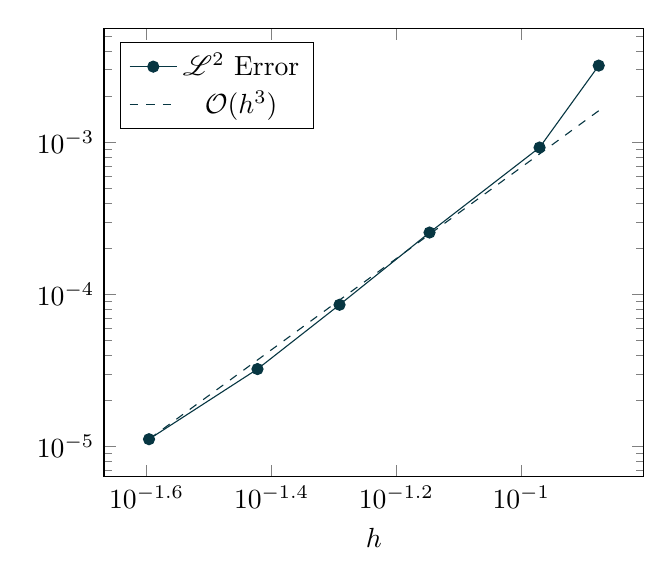
\begin{tikzpicture}
\begin{loglogaxis}[
    xlabel={$h$},
    legend pos=north west,
]

\addplot[solarized-base02, mark=*] coordinates {(0.13307,0.00319602) (0.106989,0.000923928) (0.0713092,0.000254932) (0.0511671,8.53632e-05) (0.0378115,3.22414e-05) (0.0253431,1.11436e-05)};
\addlegendentry{$\LT$ Error}

\addplot[solarized-base02, dashed] coordinates {(0.13307,0.0016131946519815491) (0.0253431,1.11436e-05)};
\addlegendentry{$\mathcal{O}(h^{3})$}

\end{loglogaxis}
\end{tikzpicture}
\end{subfigure}
\hfill
\begin{subfigure}[b]{0.45\textwidth}
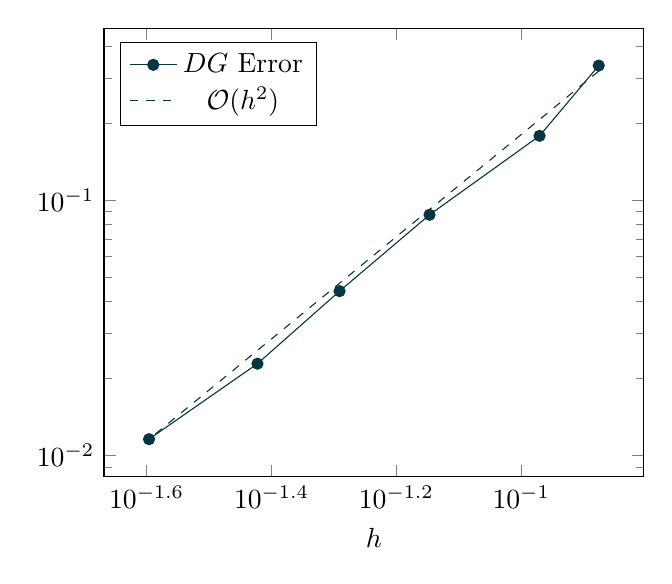
\begin{tikzpicture}
\begin{loglogaxis}[
    xlabel={$h$},
    legend pos=north west,
]

\addplot[solarized-base02, mark=*] coordinates {(0.13307,0.335441) (0.106989,0.178159) (0.0713092,0.087464) (0.0511671,0.0439649) (0.0378115,0.0228686) (0.0253431,0.0115813)};
\addlegendentry{$DG$ Error}

\addplot[solarized-base02, dashed] coordinates {(0.13307,0.3192994356314801) (0.0253431,0.0115813)};
\addlegendentry{$\mathcal{O}(h^{2})$}

\end{loglogaxis}
\end{tikzpicture}
\end{subfigure}
    % Errors v Size template for TikZ.

\begin{subfigure}[b]{0.45\textwidth}
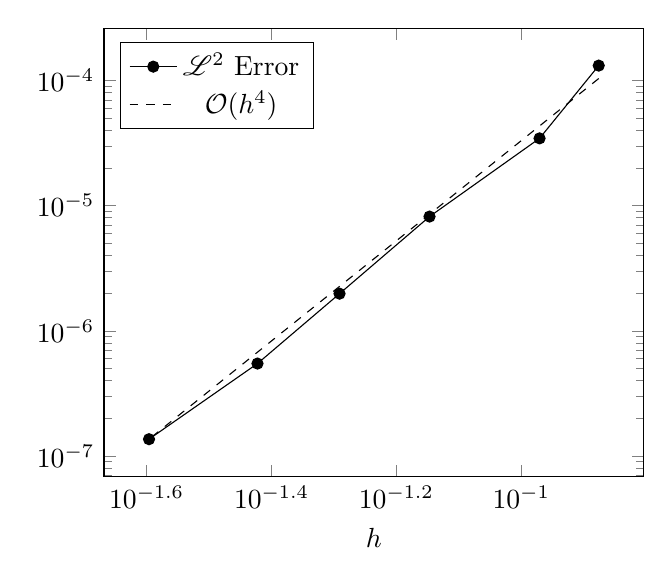
\begin{tikzpicture}
\begin{loglogaxis}[
    xlabel={$h$},
    legend pos=north west,
]

\addplot[black, mark=*] coordinates {(0.13307,0.000131393) (0.106989,3.44649e-05) (0.0713092,8.1769e-06) (0.0511671,1.98114e-06) (0.0378115,5.47747e-07) (0.0253431,1.36302e-07)};
\addlegendentry{$\LT$ Error}

\addplot[black, dashed] coordinates {(0.13307,0.0001036057614569891) (0.0253431,1.36302e-07)};
\addlegendentry{$\mathcal{O}(h^{4})$}

\end{loglogaxis}
\end{tikzpicture}
\end{subfigure}
\hfill
\begin{subfigure}[b]{0.45\textwidth}
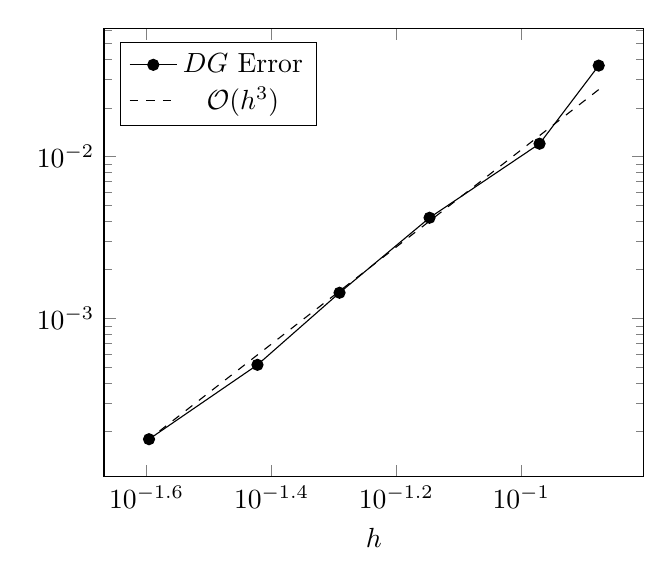
\begin{tikzpicture}
\begin{loglogaxis}[
    xlabel={$h$},
    legend pos=north west,
]

\addplot[black, mark=*] coordinates {(0.13307,0.036557) (0.106989,0.0120258) (0.0713092,0.00419264) (0.0511671,0.00144215) (0.0378115,0.000517054) (0.0253431,0.000179452)};
\addlegendentry{$DG$ Error}

\addplot[black, dashed] coordinates {(0.13307,0.025978230256595083) (0.0253431,0.000179452)};
\addlegendentry{$\mathcal{O}(h^{3})$}

\end{loglogaxis}
\end{tikzpicture}
\end{subfigure}
    \caption{$\LT$ and $DG$ errors versus mesh size on a sequence of uniform meshes over a square domain. $k = 2$ (top), $k = 3$ (bottom), with $N \in \{125, 250, \dots, 4000\}$.}
\end{figure}

\newpage
\begin{figure}[!ht]
    % Errors v Size template for TikZ.

\begin{subfigure}[b]{0.45\textwidth}
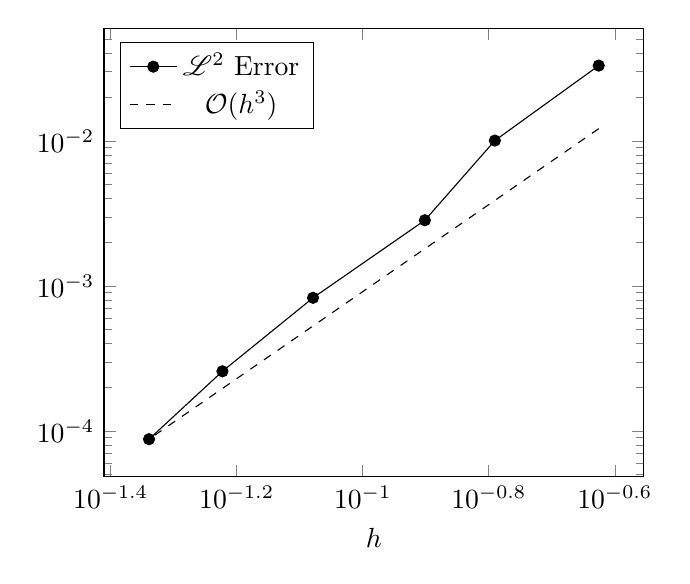
\begin{tikzpicture}
\begin{loglogaxis}[
    xlabel={$h$},
    legend pos=north west,
]

\addplot[black, mark=*] coordinates {(0.236846,0.033079) (0.162063,0.0100577) (0.125487,0.00284011) (0.0834066,0.000829064) (0.0598985,0.000258195) (0.0458041,8.78696e-05)};
\addlegendentry{$\LT$ Error}

\addplot[black, dashed] coordinates {(0.236846,0.012148530558035811) (0.0458041,8.78696e-05)};
\addlegendentry{$\mathcal{O}(h^{3})$}

\end{loglogaxis}
\end{tikzpicture}
\end{subfigure}
\hfill
\begin{subfigure}[b]{0.45\textwidth}
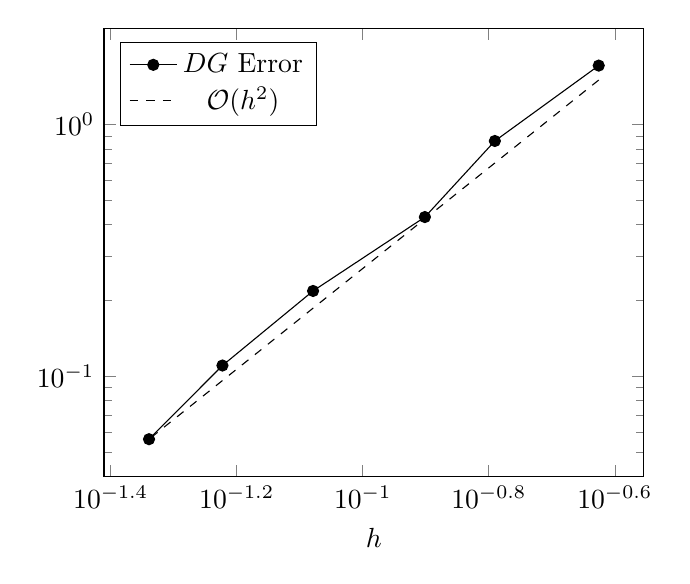
\begin{tikzpicture}
\begin{loglogaxis}[
    xlabel={$h$},
    legend pos=north west,
]

\addplot[black, mark=*] coordinates {(0.236846,1.71328) (0.162063,0.859474) (0.125487,0.428497) (0.0834066,0.217901) (0.0598985,0.110162) (0.0458041,0.0561394)};
\addlegendentry{$DG$ Error}

\addplot[black, dashed] coordinates {(0.236846,1.501036204482293) (0.0458041,0.0561394)};
\addlegendentry{$\mathcal{O}(h^{2})$}

\end{loglogaxis}
\end{tikzpicture}
\end{subfigure}
    % Errors v Size template for TikZ.

\begin{subfigure}[b]{0.45\textwidth}
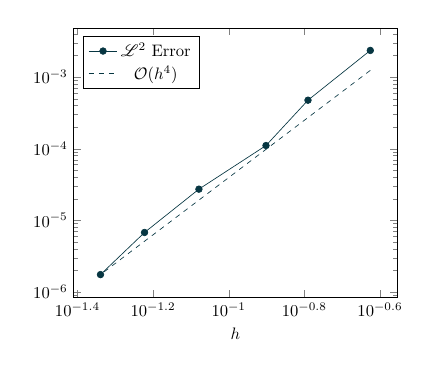
\begin{tikzpicture}[scale=.6]
\begin{loglogaxis}[
    xlabel={$h$},
    legend pos=north west,
]

\addplot[solarized-base02, mark=*] coordinates {(0.236846,0.00236589) (0.162063,0.000476832) (0.125487,0.000110835) (0.0834066,2.72149e-05) (0.0598985,6.75002e-06) (0.0458041,1.74035e-06)};
\addlegendentry{$\LT$ Error}

\addplot[solarized-base02, dashed] coordinates {(0.236846,0.0012441805245544592) (0.0458041,1.74035e-06)};
\addlegendentry{$\mathcal{O}(h^{4})$}

\end{loglogaxis}
\end{tikzpicture}
\end{subfigure}
\hfill
\begin{subfigure}[b]{0.45\textwidth}
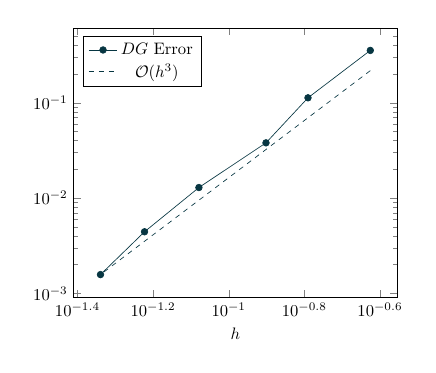
\begin{tikzpicture}[scale=.6]
\begin{loglogaxis}[
    xlabel={$h$},
    legend pos=north west,
]

\addplot[solarized-base02, mark=*] coordinates {(0.236846,0.354304) (0.162063,0.112679) (0.125487,0.0379581) (0.0834066,0.0128848) (0.0598985,0.00442298) (0.0458041,0.0015715)};
\addlegendentry{$DG$ Error}

\addplot[solarized-base02, dashed] coordinates {(0.236846,0.2172698609297559) (0.0458041,0.0015715)};
\addlegendentry{$\mathcal{O}(h^{3})$}

\end{loglogaxis}
\end{tikzpicture}
\end{subfigure}
    \caption{$\LT$ and $DG$ errors versus mesh size on a sequence of uniform meshes over an L-shaped domain. $k = 2$ (top), $k = 3$ (bottom), with $N \in \{125, 250, \dots, 4000\}$.}
\end{figure}

\newpage
\subsubsection{Meshes}

\begin{figure}[!ht]
	\centering
	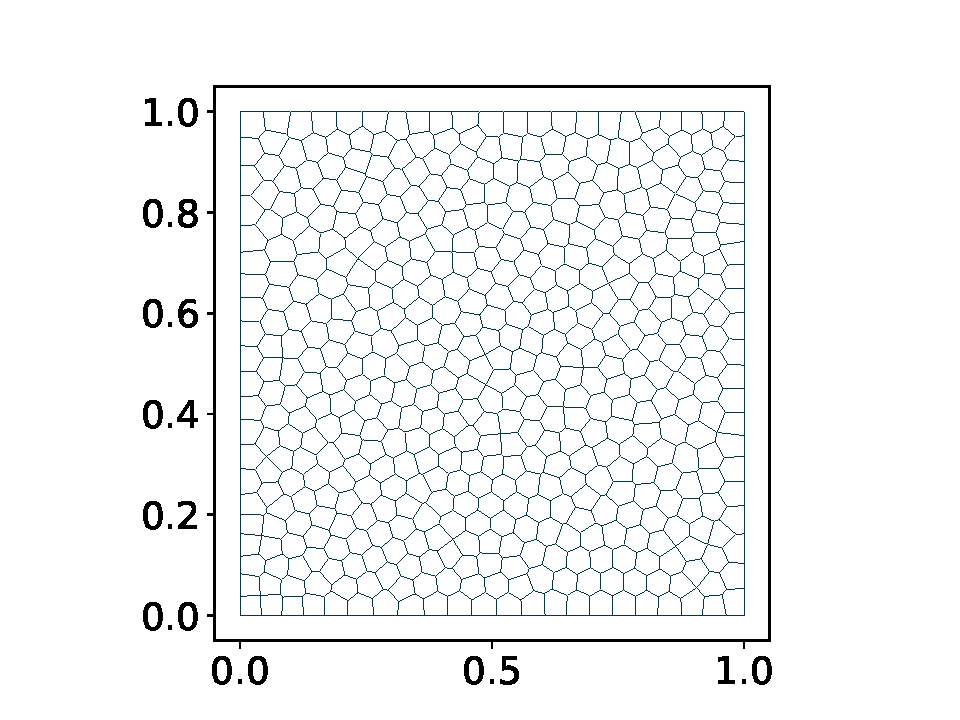
\includegraphics[trim=1cm 0.5cm 1cm 0.5cm, clip, width=0.3\textwidth]{meshes/uniform/square_500.pdf}
	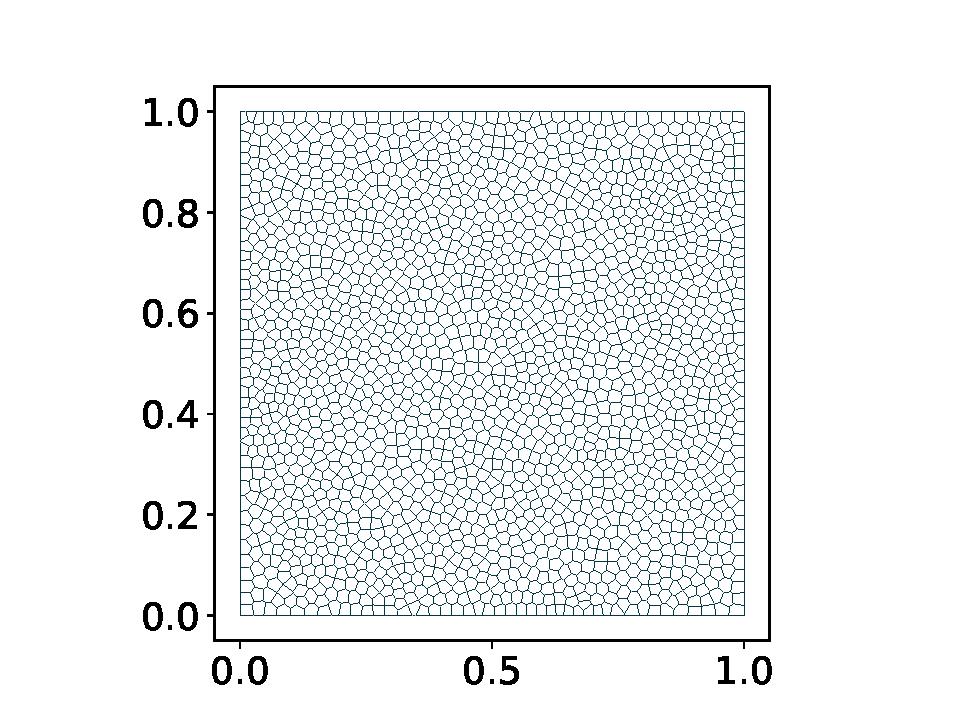
\includegraphics[trim=1cm 0.5cm 1cm 0.5cm, clip, width=0.3\textwidth]{meshes/uniform/square_2000.pdf}
	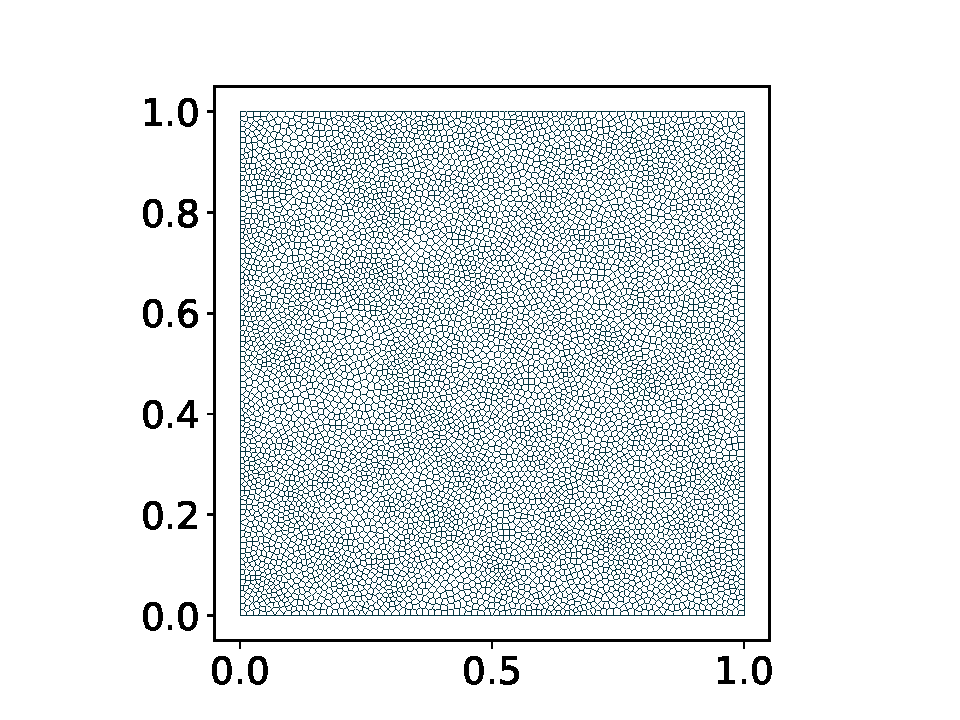
\includegraphics[trim=1cm 0.5cm 1cm 0.5cm, clip, width=0.3\textwidth]{meshes/uniform/square_8000.pdf}
	\caption{Square uniform meshes, with $N \in \{500, 2000, 8000\}$.}
\end{figure}

\begin{figure}[!ht]
	\centering
	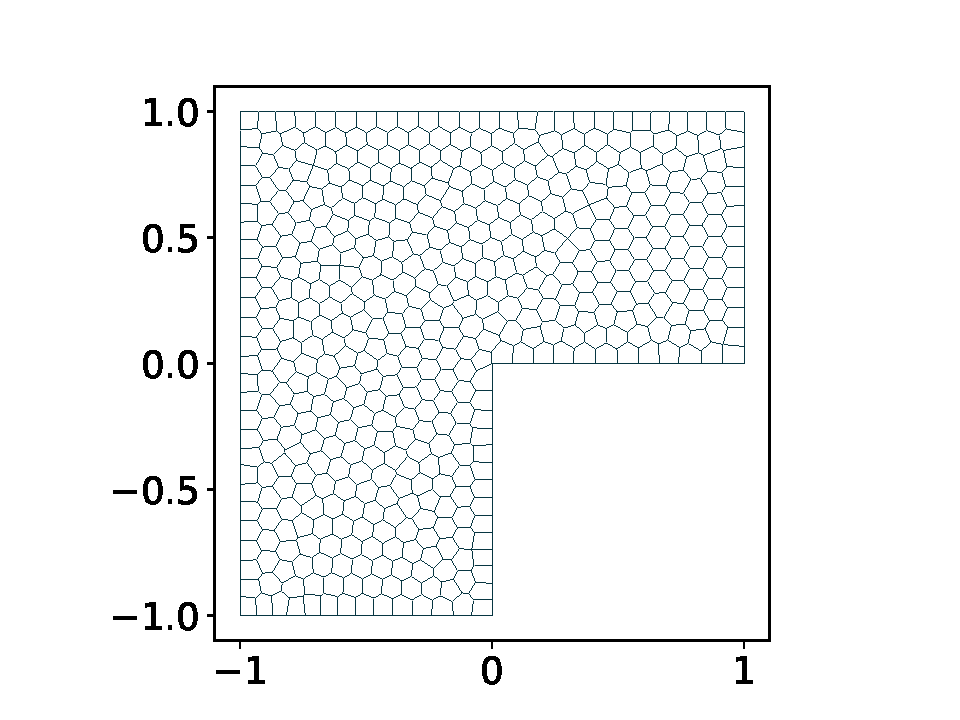
\includegraphics[trim=1cm 0.5cm 1cm 0.5cm, clip, width=0.3\textwidth]{meshes/uniform/lshape_500.pdf}
	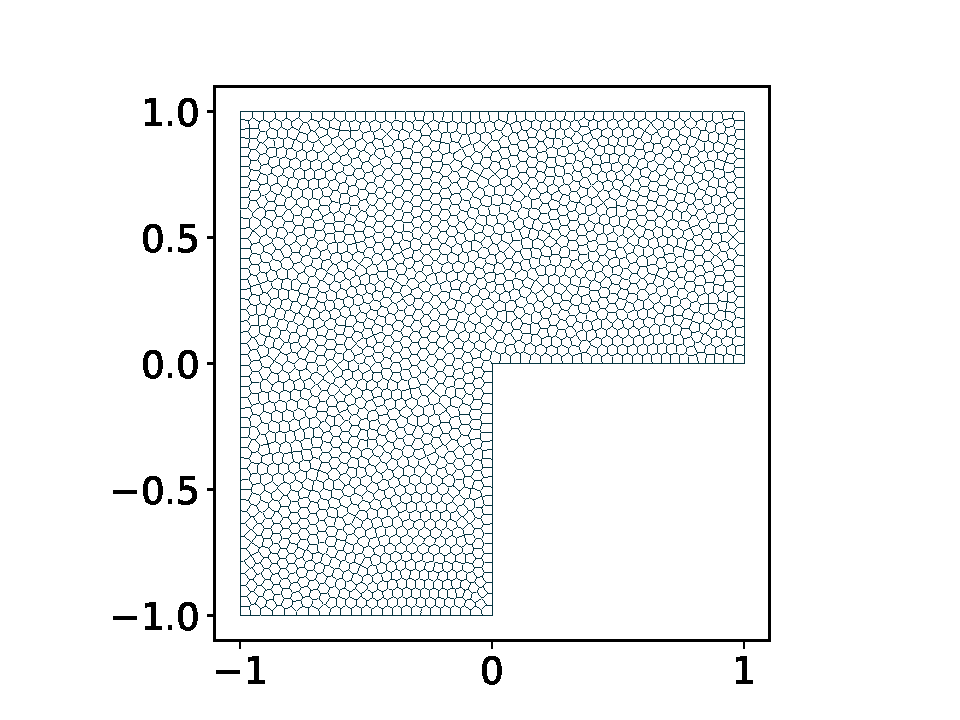
\includegraphics[trim=1cm 0.5cm 1cm 0.5cm, clip, width=0.3\textwidth]{meshes/uniform/lshape_2000.pdf}
	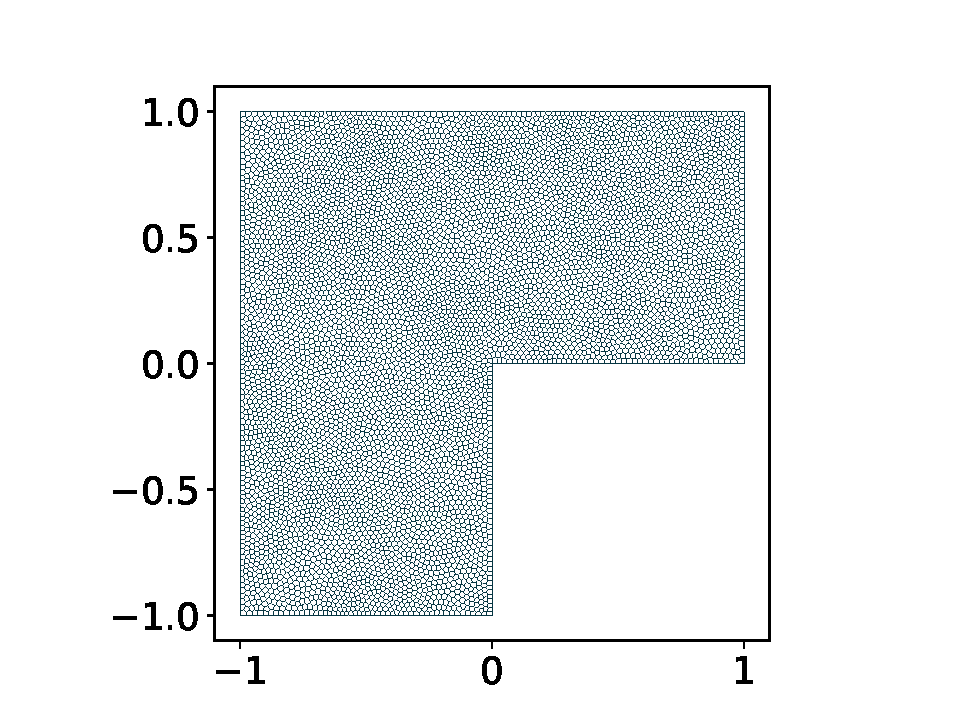
\includegraphics[trim=1cm 0.5cm 1cm 0.5cm, clip, width=0.3\textwidth]{meshes/uniform/lshape_8000.pdf}
	\caption{L-shaped uniform meshes, with $N \in \{500, 2000, 8000\}$.}
\end{figure}

\newpage
\subsection{Pathological solutions}

Tests over a sequence of uniform meshes, using pathological functions as exact solutions, highlight the need for an adaptive algorithm.

\cite{Antonietti2013} The pathological function for the square domain is:

\begin{gather} \label{pathological_square}
    u(x, y) = \frac{1 - e^{-100x}}{1 - e^{-100}} \sin(\pi y) (1 - x),
\end{gather}

which exhibits a strong boundary layer along the line $x = 0$.

For the L-shaped domain, the pathological function is:

\begin{gather} \label{pathological_lshape}
    u(\rho, \theta) = \rho^{2 / 3} \sin\left(\frac{2 \theta}{3}\right),
\end{gather}

where $f = 0$ and $u$ is analytical in $\Omega \setminus \Vector{0}$, but $\grad{u}$ is singular at the origin.

Error trends are discussed in the following sections.

\newpage
\subsubsection{Errors}

Despite being a smooth function, the pathological solution over the square domain achieves the expected convergence rate, albeit at a slower pace.

\begin{figure}[!ht]
    % Errors v Size template for TikZ.

\begin{subfigure}[b]{0.45\textwidth}
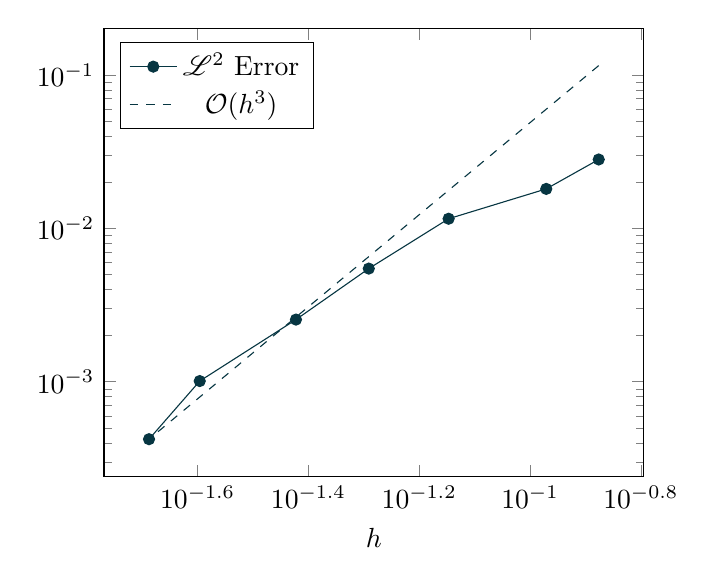
\begin{tikzpicture}
\begin{loglogaxis}[
    xlabel={$h$},
    legend pos=north west,
]

\addplot[solarized-base02, mark=*] coordinates {(0.13307,0.0281162) (0.106989,0.0180826) (0.0713092,0.0115527) (0.0511671,0.00546711) (0.0378115,0.00254289) (0.0253431,0.00101081) (0.0205266,0.000422415)};
\addlegendentry{$\LT$ Error}

\addplot[solarized-base02, dashed] coordinates {(0.13307,0.11508765584587866) (0.0205266,0.000422415)};
\addlegendentry{$\mathcal{O}(h^{3})$}

\end{loglogaxis}
\end{tikzpicture}
\end{subfigure}
\hfill
\begin{subfigure}[b]{0.45\textwidth}
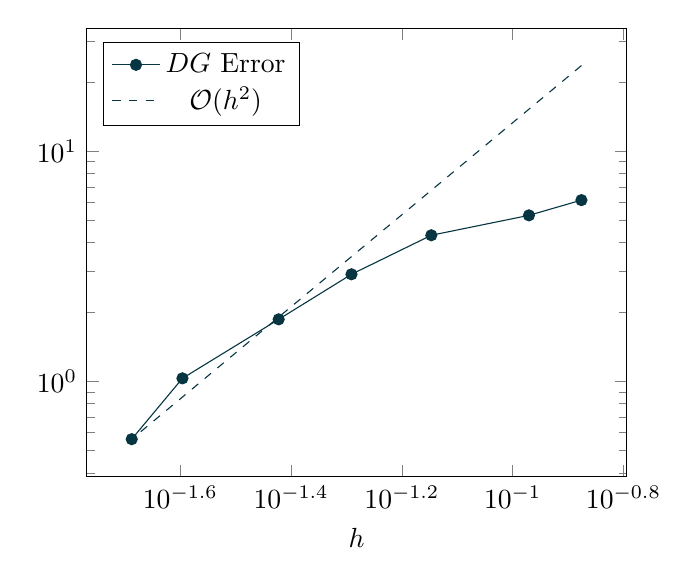
\begin{tikzpicture}
\begin{loglogaxis}[
    xlabel={$h$},
    legend pos=north west,
]

\addplot[solarized-base02, mark=*] coordinates {(0.13307,6.12566) (0.106989,5.25995) (0.0713092,4.30988) (0.0511671,2.91652) (0.0378115,1.85839) (0.0253431,1.02974) (0.0205266,0.5601)};
\addlegendentry{$DG$ Error}

\addplot[solarized-base02, dashed] coordinates {(0.13307,23.539208068455636) (0.0205266,0.5601)};
\addlegendentry{$\mathcal{O}(h^{2})$}

\end{loglogaxis}
\end{tikzpicture}
\end{subfigure}
    % Errors v Size template for TikZ.

\begin{subfigure}[b]{0.45\textwidth}
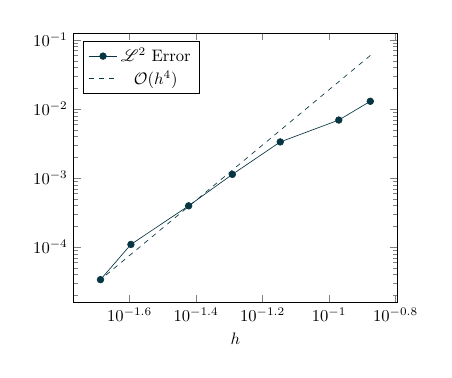
\begin{tikzpicture}[scale=.6]
\begin{loglogaxis}[
    xlabel={$h$},
    legend pos=north west,
]

\addplot[solarized-base02, mark=*] coordinates {(0.13307,0.0129373) (0.106989,0.00691892) (0.0713092,0.00333505) (0.0511671,0.0011295) (0.0378115,0.000395856) (0.0253431,0.000109201) (0.0205266,3.37306e-05)};
\addlegendentry{$\LT$ Error}

\addplot[solarized-base02, dashed] coordinates {(0.13307,0.05957672373397235) (0.0205266,3.37306e-05)};
\addlegendentry{$\mathcal{O}(h^{4})$}

\end{loglogaxis}
\end{tikzpicture}
\end{subfigure}
\hfill
\begin{subfigure}[b]{0.45\textwidth}
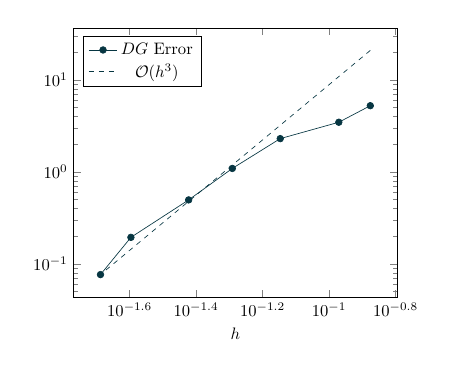
\begin{tikzpicture}[scale=.6]
\begin{loglogaxis}[
    xlabel={$h$},
    legend pos=north west,
]

\addplot[solarized-base02, mark=*] coordinates {(0.13307,5.22824) (0.106989,3.45593) (0.0713092,2.29411) (0.0511671,1.08811) (0.0378115,0.495229) (0.0253431,0.194102) (0.0205266,0.0764724)};
\addlegendentry{$DG$ Error}

\addplot[solarized-base02, dashed] coordinates {(0.13307,20.83503013128883) (0.0205266,0.0764724)};
\addlegendentry{$\mathcal{O}(h^{3})$}

\end{loglogaxis}
\end{tikzpicture}
\end{subfigure}
    \caption{$\LT$ and $DG$ errors versus mesh size on a sequence of uniform meshes over a square domain. $k = 2$ (top), $k = 3$ (bottom), with $N \in \{125, 250, \dots, 8000\}$.}
\end{figure}

\newpage

Due to its nature, the pathological solution on the L-shaped domain does not reach the expected convergence rate. The expected convergence rate, given its Sobolev regularity, is:

\begin{gather}
    \lVert u - u^k_h \rVert_{DG} \approx h^{2/3}.
\end{gather}

\begin{figure}[!ht]
    % Errors v Size template for TikZ.

\begin{subfigure}[b]{0.45\textwidth}
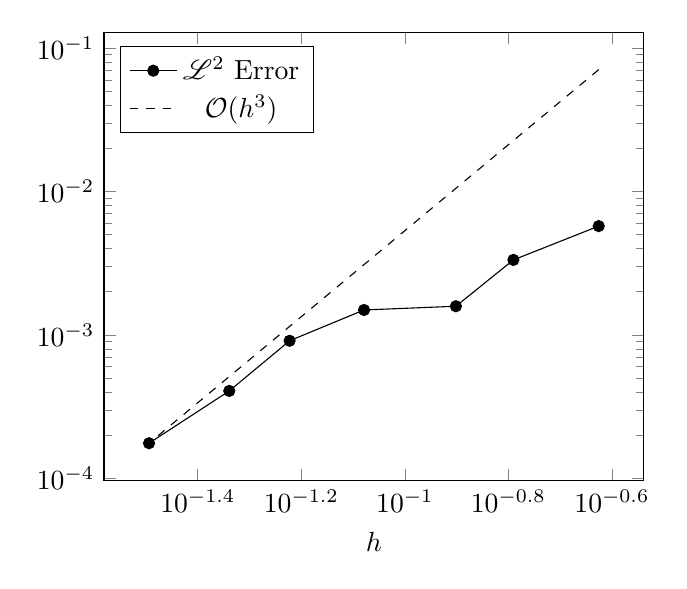
\begin{tikzpicture}
\begin{loglogaxis}[
    xlabel={$h$},
    legend pos=north west,
]

\addplot[black, mark=*] coordinates {(0.236846,0.00573887) (0.162063,0.00333593) (0.125487,0.00158497) (0.0834066,0.00149286) (0.0598985,0.000910291) (0.0458041,0.000406812) (0.0320544,0.000175592)};
\addlegendentry{$\LT$ Error}

\addplot[black, dashed] coordinates {(0.236846,0.07083370080315939) (0.0320544,0.000175592)};
\addlegendentry{$\mathcal{O}(h^{3})$}

\end{loglogaxis}
\end{tikzpicture}
\end{subfigure}
\hfill
\begin{subfigure}[b]{0.45\textwidth}
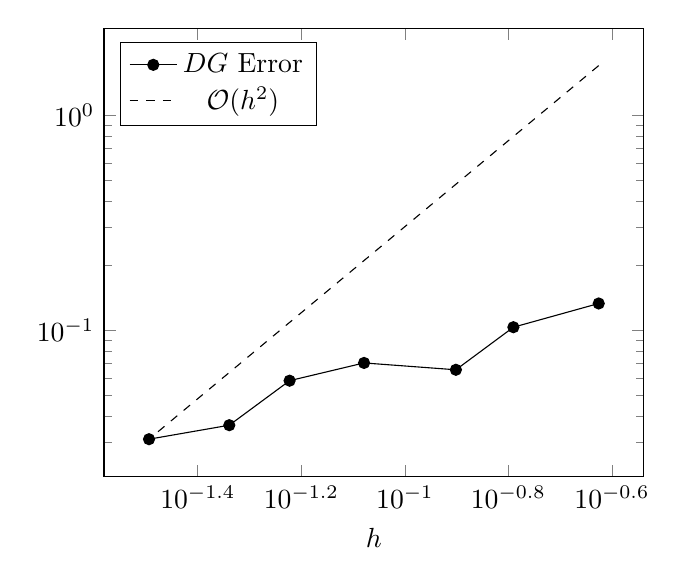
\begin{tikzpicture}
\begin{loglogaxis}[
    xlabel={$h$},
    legend pos=north west,
]

\addplot[black, mark=*] coordinates {(0.236846,0.13327) (0.162063,0.103364) (0.125487,0.0655286) (0.0834066,0.0705169) (0.0598985,0.0583046) (0.0458041,0.0362069) (0.0320544,0.0311668)};
\addlegendentry{$DG$ Error}

\addplot[black, dashed] coordinates {(0.236846,1.7015668612169044) (0.0320544,0.0311668)};
\addlegendentry{$\mathcal{O}(h^{2})$}

\end{loglogaxis}
\end{tikzpicture}
\end{subfigure}
    % Errors v Size template for TikZ.

\begin{subfigure}[b]{0.45\textwidth}
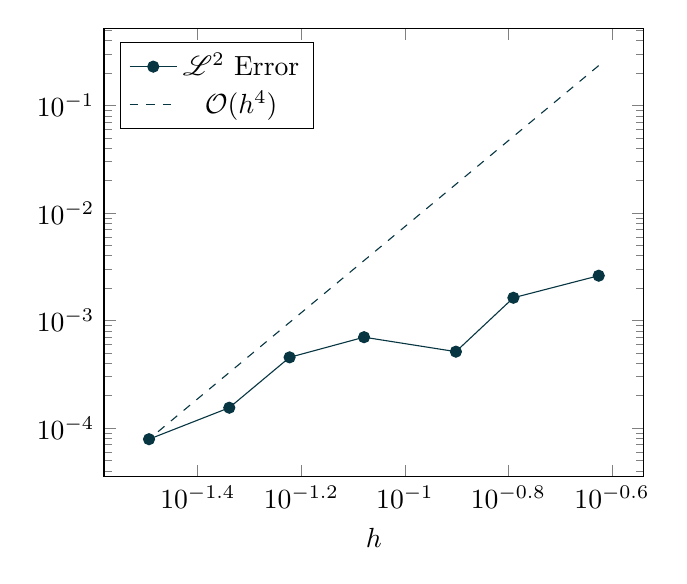
\begin{tikzpicture}
\begin{loglogaxis}[
    xlabel={$h$},
    legend pos=north west,
]

\addplot[solarized-base02, mark=*] coordinates {(0.236846,0.00261101) (0.162063,0.00162784) (0.125487,0.000513351) (0.0834066,0.000699775) (0.0598985,0.000454435) (0.0458041,0.000154545) (0.0320544,7.87786e-05)};
\addlegendentry{$\LT$ Error}

\addplot[solarized-base02, dashed] coordinates {(0.236846,0.23481285454935658) (0.0320544,7.87786e-05)};
\addlegendentry{$\mathcal{O}(h^{4})$}

\end{loglogaxis}
\end{tikzpicture}
\end{subfigure}
\hfill
\begin{subfigure}[b]{0.45\textwidth}
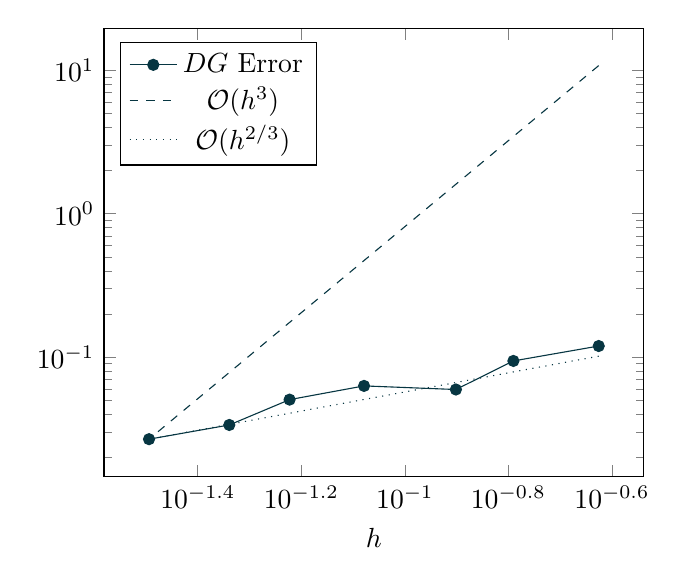
\begin{tikzpicture}
\begin{loglogaxis}[
    xlabel={$h$},
    legend pos=north west,
]

\addplot[solarized-base02, mark=*] coordinates {(0.236846,0.119546) (0.162063,0.0940845) (0.125487,0.0594576) (0.0834066,0.0630073) (0.0598985,0.0505441) (0.0458041,0.0336456) (0.0320544,0.0267768)};
\addlegendentry{$DG$ Error}

\addplot[solarized-base02, dashed] coordinates {(0.236846,10.801744041106874) (0.0320544,0.0267768)};
\addlegendentry{$\mathcal{O}(h^{3})$}

\addplot[solarized-base02, dotted] coordinates {(0.236846,0.10158063960750381) (0.0320544,0.0267768)};
\addlegendentry{$\mathcal{O}(h^{2/3})$}

\end{loglogaxis}
\end{tikzpicture}
\end{subfigure}
    \caption{$\LT$ and $DG$ errors versus mesh size on a sequence of uniform meshes over an L-shaped domain. $k = 2$ (top), $k = 3$ (bottom), with $N \in \{125, 250, \dots, 8000\}$.}
\end{figure}

	\newpage
    \section{Implementing the \textit{h-Adaptivity}}
	\subsection{A priori error estimates}

The need for \textit{h-adaptivity} arises from the inefficiency encountered solving the Poisson problem over sequences of uniform meshes while working with pathological exact solutions such as \eqref{pathological_square} and \eqref{pathological_lshape}.

The first step to implement \textit{h-adaptivity} is to evaluate the $\LT$ error on each element and then refine the element with the highest error according to a specific refinement strategy.

The strategy of choice can be outlined as follows:

\begin{enumerate}
    \item For polygons with $N_e \leq 4$, the refiner adds a single node at the polygon's centroid and then connects each edge's midpoint to this new node, creating $N_e$ new quadrilaterals.
    \item For polygons with $N_e > 4$, the refiner adds $N_e$ new nodes at the midpoints of the segments connecting the polygon's centroid to the midpoints of its edges. The refiner then connects these points to form quadrilaterals along the polygon's edges and creates a new smaller polygon by connecting all the new internal nodes.
\end{enumerate}

Refinement occurs by setting a refinement percentage and marking all elements where the local error exceeds that percentage of the highest error.

Error trends and refined meshes in the following pages.

\newpage
\subsubsection{Errors}

The following plots demonstrate that the adaptive approach (black) significantly outperforms uniform refinement (blue) when handling these pathological solutions\footnote{$N \in \{125, 250, \dots, 8000\}$ for the uniform meshes.}.

\begin{figure}[!ht]
	\begin{subfigure}[b]{0.45\textwidth}
		% Errors v DOFs template for TikZ.

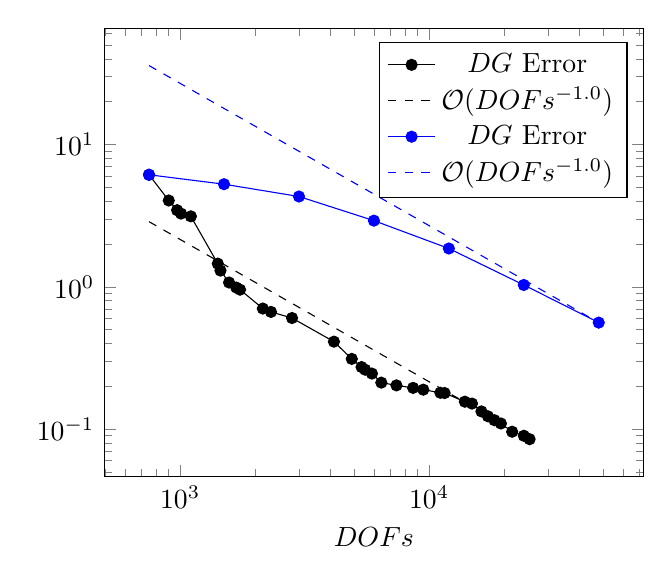
\begin{tikzpicture}
\begin{loglogaxis}[
    xlabel={$DOFs$},
    legend pos=north east,
]

\addplot[black, mark=*] coordinates {(750,6.12566) (900,4.03955) (972,3.45362) (1008,3.26799) (1104,3.12636) (1416,1.45431) (1452,1.30003) (1572,1.0716) (1680,0.987916) (1740,0.954643) (2148,0.70325) (2316,0.666102) (2814,0.603387) (4146,0.411693) (4890,0.311397) (5352,0.272847) (5532,0.261592) (5892,0.245583) (6426,0.212127) (7392,0.202913) (8622,0.194848) (9474,0.189286) (11094,0.180045) (11538,0.179227) (13914,0.155865) (14862,0.151127) (16218,0.133144) (17226,0.123047) (18294,0.11549) (19422,0.109519) (21546,0.0958461) (24006,0.0897779) (25320,0.0849597)};
\addlegendentry{$DG$ Error}

\addplot[black, dashed] coordinates {(750,2.868239472) (25320,0.0849597)};
\addlegendentry{$\mathcal{O}(DOFs^{-1.0})$}

\addplot[blue, mark=*] coordinates {(750,6.12566) (1500,5.25995) (3000,4.30988) (6000,2.91652) (12000,1.85839) (24000,1.02974) (48000,0.5601)};
\addlegendentry{$DG$ Error}

\addplot[blue, dashed] coordinates {(750,35.8464) (48000,0.5601)};
\addlegendentry{$\mathcal{O}(DOFs^{-1.0})$}

\end{loglogaxis}
\end{tikzpicture}
	\end{subfigure}
	% \begin{subfigure}[b]{0.45\textwidth}
	% 	% Errors v DOFs template for TikZ.

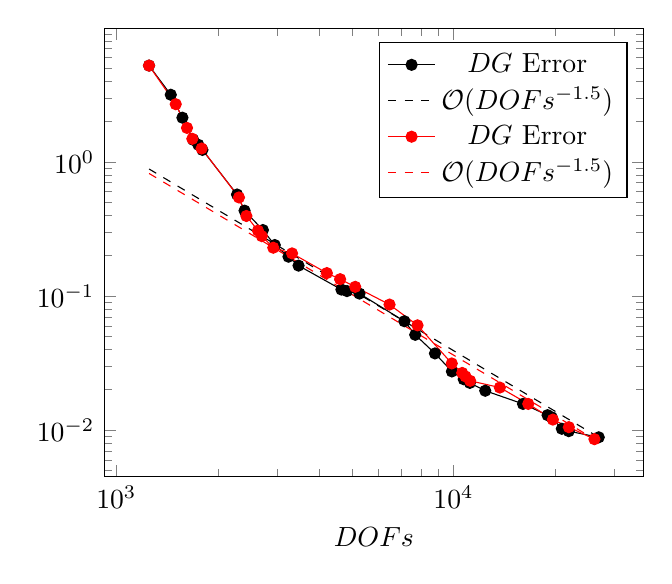
\begin{tikzpicture}
\begin{loglogaxis}[
    xlabel={$DOFs$},
    legend pos=north east,
]

\addplot[black, mark=*] coordinates {(1250,5.22824) (1450,3.16847) (1570,2.13764) (1690,1.46207) (1750,1.34315) (1800,1.22937) (2280,0.571535) (2400,0.433165) (2720,0.310514) (2950,0.239953) (3240,0.196515) (3470,0.168581) (4650,0.111757) (4830,0.108861) (5260,0.104274) (7150,0.0648557) (7700,0.0513934) (8810,0.0373304) (9890,0.0273954) (10720,0.0239574) (11180,0.0225082) (12420,0.0196702) (16070,0.0156938) (19010,0.0129343) (19560,0.0124709) (20950,0.0102387) (21970,0.00982763) (26960,0.00884522)};
\addlegendentry{$DG$ Error}

\addplot[black, dashed] coordinates {(1250,0.8859790477668384) (26960,0.00884522)};
\addlegendentry{$\mathcal{O}(DOFs^{-1.5})$}

\addplot[red, mark=*] coordinates {(1250,5.22824) (1500,2.69514) (1620,1.7934) (1680,1.48702) (1790,1.25894) (2310,0.543447) (2430,0.395368) (2630,0.307434) (2700,0.279644) (2920,0.229209) (3320,0.207952) (4210,0.148303) (4610,0.133591) (5110,0.117099) (6460,0.0863494) (7820,0.0604748) (9880,0.0314321) (10610,0.0267064) (10850,0.0251548) (11200,0.0233236) (13720,0.0207803) (16660,0.0156883) (19710,0.0119851) (21980,0.0105234) (26180,0.00856227)};
\addlegendentry{$DG$ Error}

\addplot[red, dashed] coordinates {(1250,0.8206885275389775) (26180,0.00856227)};
\addlegendentry{$\mathcal{O}(DOFs^{-1.5})$}

\end{loglogaxis}
\end{tikzpicture}
	% \end{subfigure}
    \caption{$DG$ errors vs $DOFs$ comparison between adaptively refined meshes and a sequence of uniform meshes over a square domain. $k = 2$ (left), $k = 3$ (right).}
\end{figure}

\newpage
\subsubsection{Meshes}

Due to localized errors, the meshes are refined in areas where the error is greatest, thereby minimizing the number of degrees of freedom in regions where the solution is already well-approximated.

% \begin{figure}[!ht]
% 	\centering
	
% 	% TBA

% 	\caption{Square mesh after 2, 4 and 6 refinements, $N_0 = 100$.}
% \end{figure}

% \begin{figure}[!ht]
% 	\centering
	
% 	% TBA

% 	\caption{L-shaped mesh after 2, 4 and 6 refinements, $N_0 = 100$.}
% \end{figure}

\newpage
\subsection{A posteriori error estimates}

The second step to implement \textit{h-adaptivity} is to define an \textit{a posteriori} error estimator, enabling the identification of elements that need refinement without requiring any information about the exact solution.

\cite{Cangiani2023} One possible approach considers the following upper bound on the error:

\begin{gather}
	\lVert u - u^k_h \rVert_{\LT(\Omega)} \leq C_{ub} \sum_{K \in \Tau_h} (R_K^2 + O_K^2),
\end{gather}

where:

\begin{gather}
	R_K^2 = R_{K, E}^2 + R_{K, N}^2 + R_{K, J}^2 + R_{K, T}^2
\end{gather}

is the local estimator and:

\begin{gather}
	O_K^2 = O_{K, E}^2 + O_{K, J}^2 + O_{K, T}^2
\end{gather}

is the local data oscillation, with each term given by:

\begin{align}
	R_{K, E} &= \lVert h (\bar{f} + \Delta u^k_h) \rVert_{\LT(K)}, \\
	R_{K, N} &= \lVert h^{1/2} \llbracket \grad u^k_h \cdot \Vector{n} \rrbracket \rVert_{\LT(\partial K)}, \\
	R^2_{K, J} &= \lVert \sigma^{1/2} \llbracket u^k_h \rrbracket \rVert^2_{\LT(\partial K \cap \Gamma_{i})} + \lVert \sigma^{1/2} (u^k_h - \bar{g}) \rVert^2_{\LT(\partial K \cap \partial \Omega)}, \\
	R^2_{K, T} &= \lVert h^{1/2} \llbracket \grad u^k_h \cdot \Vector{e} \rrbracket \rVert^2_{\LT(\partial K \cap \Gamma_{i})} + \lVert \sigma^{1/2} \grad (u^k_h - \bar{g}) \cdot \Vector{e} \rVert^2_{\LT(\partial K \cap \partial \Omega)}, \\
	O_{K, E} &= \lVert h (f - \bar{f}) \rVert_{\LT(K)}, \\
	O_{K, J} &= \lVert \sigma^{1/2} (g - \bar{g}) \rVert_{\LT(\partial K \cap \partial \Omega)}, \\
	O_{K, T} &= \lVert h^{1/2} \grad (g - \bar{g}) \cdot \Vector{e} \rVert_{\LT(\partial K \cap \partial \Omega)}.
\end{align}

Here, $h$ represents the element size, $\sigma$ denotes the penalty coefficient for a given edge, and $\Vector{e}$ represents the unit vector along a given edge for tangent gradients.

\newpage
\subsubsection{Errors}

These error trends demonstrate that the \textit{a posteriori} error estimates (red) behave similarly to the \textit{a priori} estimates (black). Additionally, in the case of the L-shaped domain, they exhibit improved behavior due to more concentrated refinement in the region of greatest interest. This is due to the significant local data oscillation caused by the singularity of $\grad u$ at the origin for this particular pathological solution.

% \begin{figure}[!ht]
% 	\centering
	
% 	% TBA

% 	\caption{Comparison of $\LT$ and DG errors versus $\text{DOFs}^{1/2}$ between two sequences of \textit{h-adaptively} refined meshes over a square domain (top) and an L-shaped domain (bottom), $k = 2$.}
% \end{figure}

\newpage
\subsubsection{Meshes}

These meshes exhibit a more concentrated refinement compared to those refined using \textit{a priori} error estimates.

% \begin{figure}[!ht]
% 	\centering
	
% 	% TBA

% 	\caption{Square mesh after 2, 4 and 6 refinements, $N_0 = 100$.}
% \end{figure}

% \begin{figure}[!ht]
% 	\centering
	
% 	% TBA

% 	\caption{L-shaped mesh after 2, 4 and 6 refinements, $N_0 = 100$.}
% \end{figure}

\newpage
\subsection{A code snippet}

Here's a snippet to illustrate the mesh size refinement from the user's perspective:

\lstinputlisting[style=cpp, firstline=11]{../snippets/h_refine.cpp}

	\newpage
    \section{Implementing the \textit{p-Adaptivity}}

	\newpage
	\addcontentsline{toc}{section}{References}
	\bibliography{bibliography/refs.bib}
	\bibliographystyle{siam}

\end{document}
